\documentclass[
	% parskip=half,
	a4paper,
]{scrarticle}

\usepackage{xcolor}
\definecolor{seeblau}{HTML}{00A9E0}
\definecolor{seegrau}{HTML}{9AA0A7}

\definecolor{seeblau1}{HTML}{CCEEF9}
\definecolor{seeblau2}{HTML}{A6E1F4}
\definecolor{seeblau3}{HTML}{59C7EB}
\definecolor{seeblau4}{HTML}{00A9E0}
\definecolor{seeblau5}{HTML}{008ECE}


\usepackage{graphicx}
\usepackage{amsmath}
\usepackage{subcaption}
\usepackage{wrapfig}
\usepackage[english]{babel}
\usepackage{blindtext}
\usepackage{microtype}
\usepackage{siunitx}
\usepackage[utf8]{inputenc}
\usepackage{csquotes}
\usepackage{nicefrac}
\usepackage[T1]{fontenc}
\usepackage{amsfonts}
\usepackage{amssymb}
\usepackage{tikz}
\usepackage{parskip}

\usepackage{libertinus, libertinust1math}
\usepackage[sfdefault]{biolinum}
\usepackage{roboto}

\setkomafont{disposition}{\normalfont\sffamily}

% set margins
\usepackage{geometry}
\geometry{
	a4paper,
	left=2.5cm,
	right=2.5cm,
	top=2.5cm,
	bottom=2.5cm
}

% caption
\usepackage{caption}
\captionsetup{
	% font={sf},
	labelfont={sf, bf, color=seeblau},
	labelsep=quad,
	labelformat=simple,
}

% links
\usepackage{hyperref}
\hypersetup{
	colorlinks=true,
	linkcolor=seeblau,
	citecolor=seeblau,
	urlcolor=seeblau,
	% hidelinks=true
}

% bibliography
\usepackage[
	style=numeric-comp, % comp = compressed 4,5,6,7 -> 4-7
	sorting=none,		% Sort by appearance
	% autocite = superscript,
	% backref=true,
	hyperref=true,
	url=true,
	maxbibnames=100
]{biblatex}

\usepackage{float}
% \floatplacement{figure}{h}
% \floatplacement{table}{H}

% loosen float placement rules
\renewcommand{\topfraction}{0.8}
\renewcommand{\bottomfraction}{.8}
\renewcommand{\textfraction}{0.1}
\renewcommand{\floatpagefraction}{.9}
% make floats less likely to be placed on a separate page
\setcounter{totalnumber}{9}
\setcounter{topnumber}{9}
\setcounter{bottomnumber}{9}

% decrease space between floats and text
\setlength{\textfloatsep}{0.25cm}
\setlength{\floatsep}{0.25cm}

% decrease space after disposition
\RedeclareSectionCommands[
	afterskip=1px
]{section, subsection, subsubsection}

\usepackage{adjustbox}

\usepackage{datetime}
\newdateformat{dotdate}{
	\twodigit{\THEDAY}.\twodigit{\THEMONTH}.\THEYEAR
}
\newdateformat{monthyeardate}{%
  \monthname[\THEMONTH] \THEYEAR}


% header and footer
\usepackage[
  markcase=noupper
]{scrlayer-scrpage}% activates pagestyle scrheadings automatically
\clearpairofpagestyles
\setkomafont{pageheadfoot}{\normalfont\sffamily}
\setkomafont{pagenumber}{\normalfont\sffamily}
% \chead*{\color{seegrau} Draft \dotdate\today}
\ofoot*{\pagemark}
\ohead*{\rightmark}


\usepackage{ifthen}
\newcommand{\markieren}[4]{
	\ifthenelse{\equal{#1}{}}{}{\adjustbox{padding=3pt, bgcolor=seeblau1, margin=-1pt}{\strut{\sffamily\robotoMedium{#1}}}\\}
  \ifthenelse{\equal{#2}{}}{}{\adjustbox{padding=3pt, bgcolor=seeblau2, margin=-1pt}{\strut{\sffamily\robotoMedium{#2}}}\\}
	\ifthenelse{\equal{#3}{}}{}{\adjustbox{padding=3pt, bgcolor=seeblau3, margin=-1pt}{\strut{\sffamily\robotoMedium{#3}}}\\}
	\ifthenelse{\equal{#4}{}}{}{\adjustbox{padding=3pt, bgcolor=seeblau4, margin=-1pt}{\strut{\sffamily\robotoMedium{#4}}}}
}

\addbibresource{../literature.bib}
\begin{document}

\author{Leon Oleschko}
\date{\dotdate\today}

\begin{titlepage}
    \sffamily
    \vspace*{3cm}
    {
        \fontsize{32}{32}
        \markieren{}{Ultrafast}{Hot Electron}{Themal Emission}
        \title{Ultrafast Hot Electron Thremal Emission}
    }
    \vspace{.25cm}\\
    {
        \Large
        Leon Oleschko\\
        supervised by Peter Baum
        \vspace{.05cm}\\
        \dotdate\today\\
        \textbf{Draft}\\
        \vspace{.05cm}\\
        \normalsize
        Projekt Praktikum\\
        Universität Konstanz
    }
    \vfill
    {
        \normalfont\normalsize
        This report details the experimental investigation of ultrafast hot electron thermal emission from graphite using a time-integrated EMCCD spectrometer. The measured spectral radiance is compared to predictions from the two-temperature model (2TM). Resulting in strong qualitative agreement with the broadband spectral shape, validating the 2TM framework in the $\SI{100}{fs}$ regime. 
        However, quantitative analysis revealed severe experimental limitations : A scaling factor indicated a systematic power loss of three orders of magnitude, primarily attributed to bad fiber coupling. Furthermore, the spectral fit was compromised by unfiltered spurious light components. Achieving high-precision absolute spectral power requires the rectification of the power loss and the implementation of a dedicated, traceable system calibration.
    }
    \vfill
    \begin{flushright}
        Available at \url{www.github.com/leoole100/projekt-praktikum}.
    \end{flushright}
\end{titlepage}

% {
% 	\sffamily
% 	\hypersetup{hidelinks}
% 	\tableofcontents
% }

\clearpage

\section{Introduction}
The study of ultrafast thermal dynamics in materials is a cornerstone of condensed matter physics, crucial for applications ranging from high-speed electronics to energy harvesting and material processing \cite{tangPlasmonicHotElectrons2020,konigHotCarrierSolar2010}. 

When materials like graphite are exposed to femtosecond laser pulses, the absorbed energy couples initially and almost exclusively to the electron gas, leading to a state where the electron temperature ($T_e$) transiently exceeds the lattice temperature ($T_l$) by several thousand Kelvin. Understanding the subsequent processes of energy transfer and thermal relaxation is essential for predicting material response at these extreme non-equilibrium conditions.

This dynamic is commonly described by the two-temperature model (2TM). The 2TM treats the electrons and the lattice as two distinct subsystems characterized by their own temperatures, coupled by an electron-phonon relaxation time ($\tau$). While simple, this model has proven highly effective in describing the subsequent relaxation of the hot electron gas on the picosecond timescale \cite{stangeHotElectronCooling2015}. Crucially, the extreme electron temperatures reached lead to broadband blackbody-like emission, or hot electron thermal radiation, which serves as a direct experimental probe for $T_e$.
This is sometimes also called ultrafast photoluminescence \cite{luiUltrafastPhotoluminescenceGraphene2010}.

The objective of this project was twofold: first, to establish a robust experimental platform for measuring this ultrafast hot electron thermal radiation from highly-excited graphite; and second, to validate the predictions of the numerical two-temperature model against the time-integrated spectral measurements. This report details the optimization of the measurement setup, the required high-sensitivity detector characterization, and the methodology used to compare the observed spectrum with the simulated model output.

This work validates the 2TM as a predictive tool in the $\SI{100}{fs}$ regime.

\section{Numerical Model}

\begin{figure}[b]
    \centering
    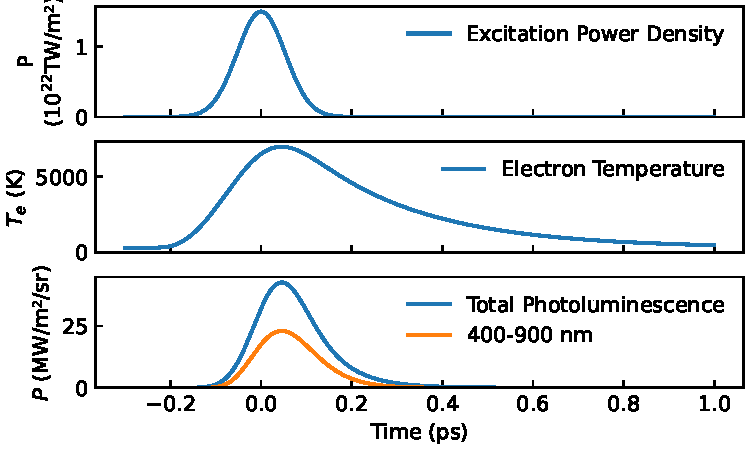
\includegraphics{../analysis/figures/model.time_evolution.pdf}
    \caption{Time evolution of the absorbed power density $P_V(t)$, the electron temperature $T_e(t)$ and the total integrated radiance $L(t)$, calculated using the two-temperature model (Eq. \ref{eq:Te}). The calculation assumes an absorbed energy density of $U_{\text{abs}} = \SI{2e9}{J/m^3}$ over a FWHM pulse with $t=\SI{250}{fs}$ and an electron-phonon coupling time of $\tau=\SI{250}{fs}$ (for graphite). The rapid temperature rise and subsequent decay illustrate the ultra-fast nature of the thermal dynamics.}
    \label{fig:timeevolution}
\end{figure}

The ultrafast thermal dynamics are modeled using a simplified two-temperature approach. An excitation pulse $P_{\text{exc}}(t)$ generates an absorbed power density $P_V(t) = P_{\text{exc}}(t) / V$ over the material's volume $V$. This input energy raises the electron temperature $T_e$, governed by the electronic heat capacity $C_e(T_e)$. Subsequently, the electrons cool via electron-phonon coupling with a relaxation time $\tau$ to the lattice at a constant temperature $T_l$.

This process is described by the ordinary differential equation:
\begin{equation}
    \frac{\mathrm d T_e(t)}{\mathrm d t}
    =
    \frac{P_V(t)}{C_e(T_e)}
    -\frac{T_e(t) - T_l}{\tau}.
    \label{eq:Te}
\end{equation}
A numerical solution based on the used excitation parameters (an absorbed energy density of $U_{\text{abs}} = \SI{2}{GJ/m^3}$ spread in a Gaussian pulse with a full width at half maximum (FWHM) of $\SI{250}{fs}$) is provided. We utilize the electronic heat capacity function from \cite{nihiraTemperatureDependenceLattice2003} and the $\tau=\SI{250}{fs}$ coupling time for graphite \cite{stangeHotElectronCooling2015}. The resulting time evolution is shown in \autoref{fig:timeevolution}.

The spectral radiance $L_\lambda$ emitted at each time step can be calculated using Planck's law:
\begin{equation}
    L_\lambda(\lambda,T)
    = \epsilon(\lambda) \frac{2hc^{2}}{\lambda^{5}}
    \frac{1}{\exp\bigl(hc / \lambda k_{\mathrm B}T\bigr)-1}.
\end{equation}
The electron gas emissivity $\epsilon$ is assumed to be unity, a common approximation for graphite \cite{sapritskyBlackbodyRadiometry1995}. The resulting time evolution of the total radiance $L=\int L_\lambda(\lambda, T) d\lambda$ and the radiance in a spectral range relevant for common detectors are also presented in \autoref{fig:timeevolution}.

\begin{figure}
    \centering
    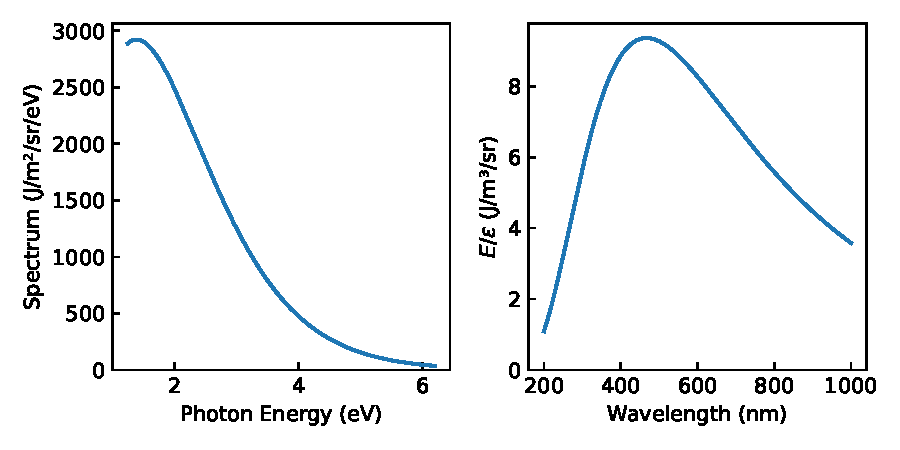
\includegraphics{../analysis/figures/model.spectrum.pdf}
    \caption{Model spectrum $H_\lambda(\lambda)$ (time-integrated spectral radiance) calculated from the time evolution shown in Figure \ref{fig:timeevolution}. The spectrum represents the total signal expected to be recorded by a time-integrating detector. Both shown over the wavelength and the photon energy.}
    \label{fig:model_spectrum}
\end{figure}

The experimentally measurable spectrum, $H_\lambda(\lambda)$, is defined as the time-integrated spectral radiance:
\begin{equation}
      H_\lambda(\lambda) = 
      \int L_\lambda\bigl(\lambda, T_e(t)\bigr)\,\mathrm dt.
\end{equation}
This is shown in \autoref{fig:model_spectrum}. We note that this spectrum can alternatively be visualized as a function of photon energy $E = h c / \lambda$. For direct comparison with the spectrometer output, however, we opt for the wavelength representation in this report.

\subsection{Sensitivity}

\begin{figure}
    \centering
    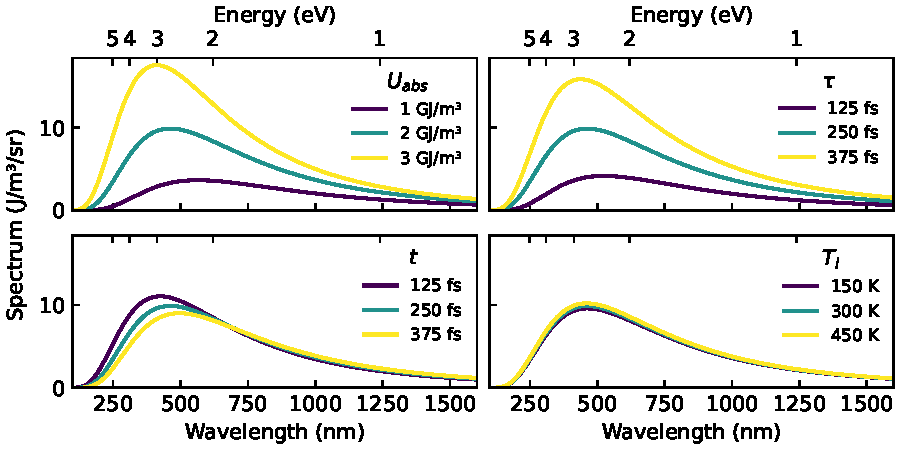
\includegraphics{../analysis/figures/sensitivity.pdf}
    \caption{Sensitivity analysis of the calculated spectrum $H_\lambda(\lambda)$ to changes in key model parameters. The results demonstrate that the absorbed energy density $U_{\text{abs}}$ and the electron-phonon coupling time $\tau$ are the dominant factors influencing the spectral shape and total emission. Conversely, variations in the pulse duration $t$ and the lattice temperature $T_l$ show only marginal impact.}
    \label{fig:sensitivity}
\end{figure}
This model is employed to study the sensitivity of the resulting spectrum to changes in the defining physical and experimental parameters. The spectrum is calculated while systematically sweeping each parameter, as detailed in \autoref{fig:sensitivity}.

The analysis reveals that the spectrum changes considerably with variations in the absorbed energy density $U_{\text{abs}}$ and the electron-phonon coupling time $\tau$. This high sensitivity emphasizes the critical importance of precisely controlling these two parameters. In contrast, changes in the excitation pulse duration $t$ and the lattice temperature $T_l$ do not significantly alter the resulting spectrum, verifying the simplifying assumption of a constant lattice temperature.

\begin{figure}
    \centering
    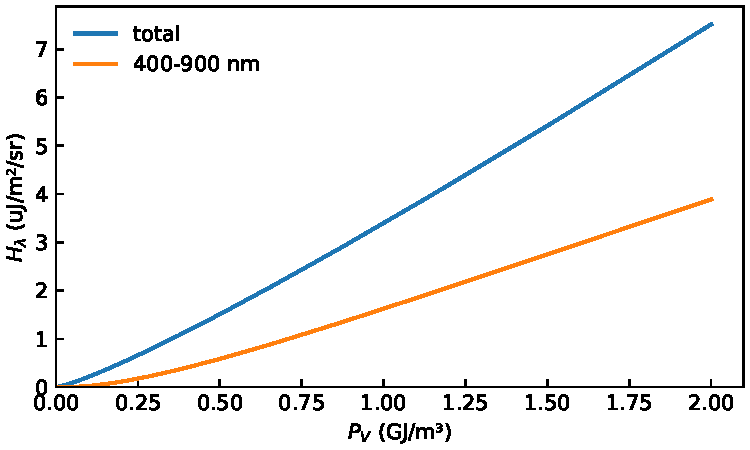
\includegraphics{../analysis/figures/powerscaling.pdf}
    \caption{Scaling behavior of the emitted thermal radiation as a function of the absorbed energy density $U_{\text{abs}}$. The scaling is shown for both the total integrated spectrum ($\int H_\lambda d\lambda$) and the radiance within the detector's spectral region. Note the non-power-law dependence, which stems from the temperature-dependent electronic heat capacity $C_e(T_e)$.}
    \label{fig:powerscaling}
\end{figure}
The dependence of the total emitted power $\int H_\lambda(\lambda) d\lambda$ on the absorbed energy density is shown in \autoref{fig:powerscaling} for both the total emission and the spectral range relevant for the detector.
The maximum reached temperature is also shown.
The total emission follows roughly a power law with a constant offset due to the non-zero lattice temperature.

\clearpage
\section{Experimental Setup}
\begin{figure}[h]
    \centering
    \begin{subfigure}{3.5in}
        \centering
        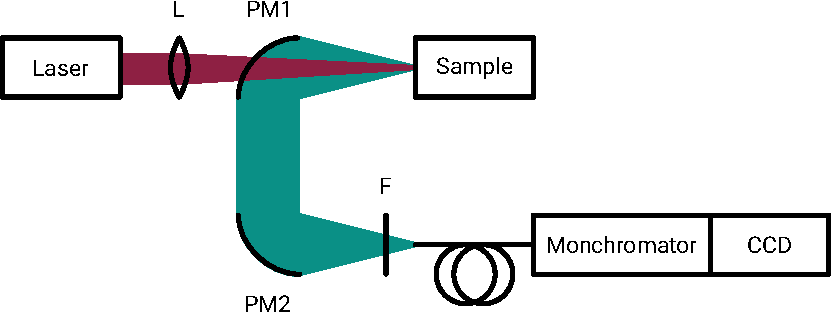
\includegraphics{figures/setup.pdf}
        \caption{Schematic}
    \end{subfigure}\hfill
    \begin{subfigure}{2in}
        \centering
        \includegraphics{figures/photo_setup.pdf}
        \caption{Photograph}
    \end{subfigure}
    \caption{Experimental setup used to measure thermal emission from ultrafast-excited hot electrons. The schematic shows the optical path and key components: L (focusing lens), PM1 and PM2 (off-axis parabolic mirrors for collection and imaging), and F (short-pass filter) used to reject scattered laser light; the photograph shows the arrangement.}
    \label{fig:setup}
\end{figure}

The experimental setup, originally developed by Leon Roob~\cite{roobThermalRadiationUltrafast2025}, is presented in \autoref{fig:setup}. It was designed to measure broadband thermal emission from hot electrons in graphite using reflective collection optics and a fibre-coupled spectrometer.

The excitation source was a Light Conversion PHAROS PH1-20 at a centre wavelength of $\SI{1030}{\nano\metre}$, with pulse duration $\SI{250}{\femto\second}$ (FWHM) and repetition rate $\SI{40}{\kilo\hertz}$. The pulse energy was $\SI{7.5}{\micro\joule}$ (average power $\SI{300}{\milli\watt}$). The beam was stabilized in four axes and expanded to a diameter of $D=\SI{5}{\milli\metre}$.

A plano-convex lens with focal length \(f=\SI{200}{\milli\metre}\) focused the beam onto the sample. The resulting spot diameter was estimated using the standard diffraction approximation \(d \approx 4\lambda f / \pi D\) to be \(\sim\SI{50}{\micro\metre}\), resulting in a fluence of \(\sim \SI{0.4}{J/cm^2}\).

The target was a graphite sample mounted on a three-axis translation stage. Thermal emission from the irradiated spot was collected by two off-axis parabolic mirrors (UV-enhanced aluminium). The first mirror (PM1, \(f=\SI{50}{\milli\metre}\)) collimated the emission; the second (PM2, \(f=\SI{101}{\milli\metre}\)) focused it onto a band-pass filter and into a multimode fibre with a $\SI{200}{\micro\metre}$ core (Ocean Optics QP200-2-SR-BX). The magnification was \(M = f_{\mathrm{PM2}}/f_{\mathrm{PM1}} = 2\), yielding an image spot of \(\sim\SI{100}{\micro\metre}\) at the fibre entrance, comfortably within the core, ensuring maximum signal collection.

The fibre fed an Acton SpectraPro 300i monochromator equipped with a 150\,lines\,mm\(^{-1}\) grating blazed at $\SI{500}{\nano\metre}$. The dispersed spectrum was detected by an Andor iXon\textsuperscript{EM}+ 897 EMCCD operated in vertical binning mode, effectively acting as a high-sensitivity 1D line detector. Wavelength calibration, performed once following the manufacturer’s procedure~\cite{roobThermalRadiationUltrafast2025}, remained stable throughout the measurements.

For optimal alignment and maximal throughput, the lens, sample, and fibre ferrule were mounted on independent precision translation stages, while the parabolic mirrors were fixed on the common optical axis.

\subsection{Noise and detector considerations}
Detecting the weak thermal radiation from hot electrons requires careful optimization of the signal-to-noise ratio (SNR). In this setup, detector-related phenomena constitute the dominant noise sources, while laser power fluctuations and mechanical variations are negligible. The underlying EMCCD noise mechanisms are well documented by Andor~\cite{dr.jowaltersSensitivityNoiseCCD2023,andorEstablishingSensitivityScientifica} and standard documents \cite{europeanmachinevisionassociationStandardCharacterizationImage2010}.

\paragraph{Readout Noise ($\sigma_{\text{read}}$)}
This is the fundamental noise from charge transfer and A/D conversion. For the present camera, the fit in \autoref{fig:dark_noise} yields a constant read noise of
\(\sigma_{\text{read}}=\SI{0.81(12)}{DN}\), consistent with the manufacturer’s specification~\cite{andorIXonEM897Manual}.
Because read noise is applied per readout cycle, utilizing hardware binning (1D line-detector mode) critically minimizes its impact by consolidating signal prior to the single read.

\paragraph{Dark Current Noise ($N_{\text{dark}}$)}
Thermally generated charge scales with temperature and time,
\(N_\text{dark}\propto \exp(-E/k_B T)\,t_\text{exp}\).
\autoref{fig:dark_noise} shows the measured dependence; fitting gives an effective activation energy \(E=\SI{0.597(4)}{eV}\).
Consequently, with the sensor cooled to $\SI{-80}{\degreeCelsius}$, the dark contribution is confirmed to be negligible for the utilized exposure times.

\begin{figure}[h]
    \centering
    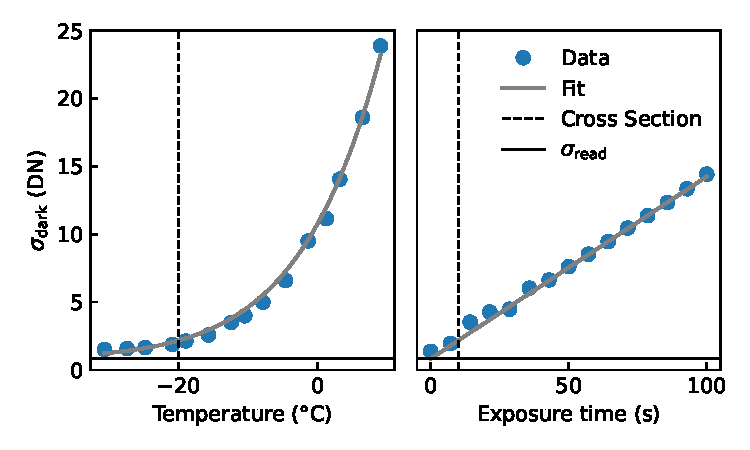
\includegraphics{../analysis/figures/dark_noise.pdf}
    \caption{Noise characterization of the EMCCD detector. The plot shows the measured noise versus sensor temperature and exposure time. The fit confirms the read noise $\sigma_{\text{read}}=\SI{0.81(12)}{e^{-}}$ and provides the effective activation energy $E=\SI{0.597(4)}{eV}$ for dark current, confirming its negligible impact at the operating temperature of \SI{-80}{\degreeCelsius}.}
    \label{fig:dark_noise}
\end{figure}

\paragraph{Clock-Induced Charge (CIC)}
CIC is created during high-speed clocking.
Its contribution scales with the electron multiplication gain; therefore, the \emph{EM gain was disabled} in this work (signal levels were well above the read-noise floor), which kept CIC negligible~\cite{andorEstablishingSensitivityScientifica}.

\paragraph{Shot Noise and System Gain ($G$)}
Under these optimized conditions (negligible $\sigma_{\text{read}}$ and $N_{\text{dark}}$), the dominant noise term is shot noise.
Incident photons create photoelectrons with quantum efficiency \(\eta\), so \(N_e=\eta\,N_{\text{photons}}\) and, for Poisson statistics, \(\operatorname{var}(N_e)=N_e\)~\cite{europeanmachinevisionassociationStandardCharacterizationImage2010}.
Let \(G\) denote the system conversion gain ($\text{DN}$ per electron). The measured signal in data numbers ($\text{DN}$) is \(S = G\,N_e\), and the measured variance becomes \(\sigma^2_{\text{meas}} \;=\; \sigma_{\text{read}}^2 \;+\; G\,S\).
Therefore, a plot of variance vs.\ mean (the photon-transfer curve) exhibits linearity in the shot-noise regime with a slope equal to $G$.
\autoref{fig:shotnoise} shows this behaviour; from the slope \(G \approx 10~\text{DN}/e^{-}\) was measured.
It is important to note that this procedure determines $G$ but \emph{not} the quantum efficiency $\eta$; it solely quantifies the Data Number-to-electron conversion.

\begin{figure}[h]
    \centering
    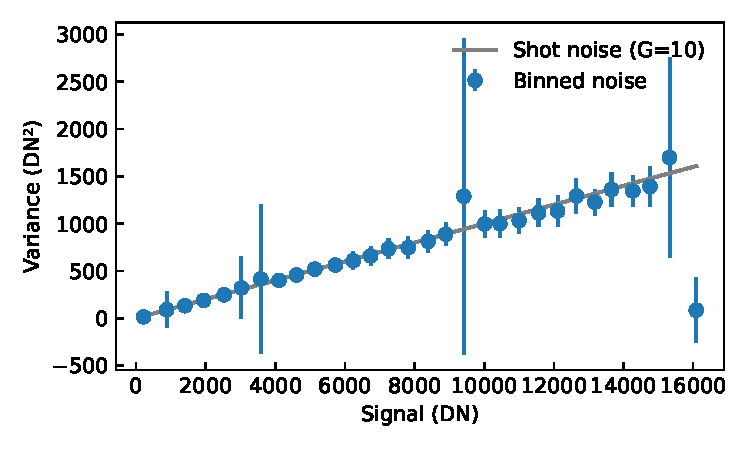
\includegraphics{../analysis/figures/shot noise.pdf}
    \caption{Photon-transfer curve (variance vs.\ mean signal) demonstrating shot-noise-limited operation under optimized conditions. The linearity of the curve confirms Poisson statistics, and the measured slope yields the system conversion gain, $G \approx 10~\text{DN}/e^{-}$.}
    \label{fig:shotnoise}
\end{figure}

\subsection{Data Processing}
All raw spectra underwent initial processing by subtracting a dark frame recorded with identical acquisition settings, a procedure which removed the fixed electronic bias and the baseline dark current contribution.

The corrected signal $S(\lambda)$ in Data Numbers ($\text{DN}$) was then converted to spectral power density $P_{\text{meas}}(\lambda)$. This conversion yields the measured signal in energy units and is performed via:
\begin{equation}
  P_{\text{meas}}(\lambda)
  = \frac{S(\lambda)}{G\,t_{\text{exp}}\,\Delta\lambda}\,\frac{hc}{\lambda},
\end{equation}
with $G$ being the system conversion gain ($\text{DN}/e^-$), $t_{\text{exp}}$ the exposure time, and $\Delta\lambda$ the spectral bin width. The final term $hc /\lambda$ converts the measured signal from electron counts per wavelength bin to the corresponding spectral power density.

\clearpage
\section{Measurement and Model Validation}

\begin{figure}[h]
    \centering
    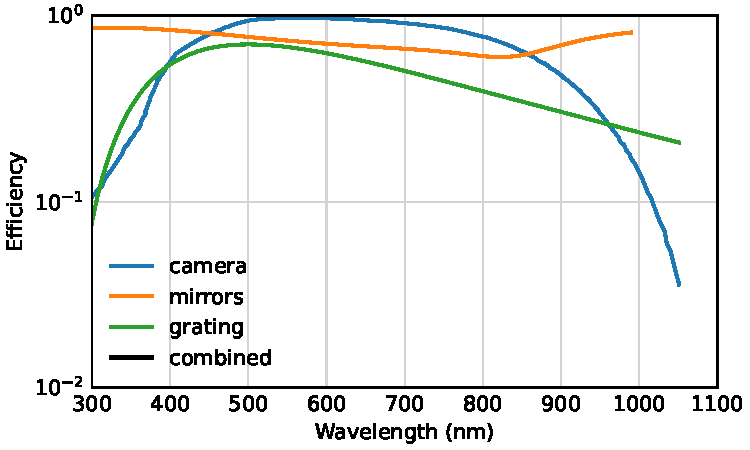
\includegraphics{../analysis/figures/combined.efficiency.pdf}
    \caption{Total spectral efficiency $\eta(\lambda)$ of the detection system, composed of the manufacturer-supplied efficiencies of the camera and mirrors, and the modeled efficiency of the grating. The unknown grating parameter $k$ is determined by fitting the integrated model to the measured spectrum, yielding $k=1.18$.}
    \label{fig:efficiency}
\end{figure}

Before the model could be compared with the experimental data, the raw spectrum (shown in \autoref{fig:fit}) was corrected using the system's spectral calibration curve. This curve, detailed in \autoref{fig:efficiency}, encapsulates the total wavelength-dependent efficiency $\eta(\lambda)$ of the detection path, encompassing: 1. The manufacturer-supplied quantum efficiency of the EMCCD camera \cite{andorIXonEM897Manual}; 2. The measured efficiencies of the reflective optics (mirrors); and 3. The efficiency of the monochromator grating. The grating efficiency, which is the most complex component, was modeled using the method proposed by Barker \cite{barkerRippleCorrectionHighdispersion1984}, incorporating a single, unknown parameter $k$ that governs the overall grating performance.

The unknown grating parameter $k$ was determined alongside two other key physical parameters—the absorbed energy density $U_{\text{abs}}$ and an overall scaling factor—by simultaneously minimizing the least-squares error between the corrected experimental spectrum and the time-integrated numerical model $H_\lambda(\lambda)$. The results of this optimization were: Grating Parameter: $k=1.18$; Fitted Absorbed Energy Density: $U_{\text{abs}} = \SI{1.35}{GJ/m^3}$; and Overall Scaling Factor: $0.72 \times 10^{-3}$. The corrected experimental spectrum, the numerical model, and the fitted parameters are displayed in \autoref{fig:fit}. While the model demonstrated a strong qualitative agreement with the measured broadband nature of the emission, a precise quantitative fit of the spectral shape proved challenging.

\begin{figure}[h]
    \centering
    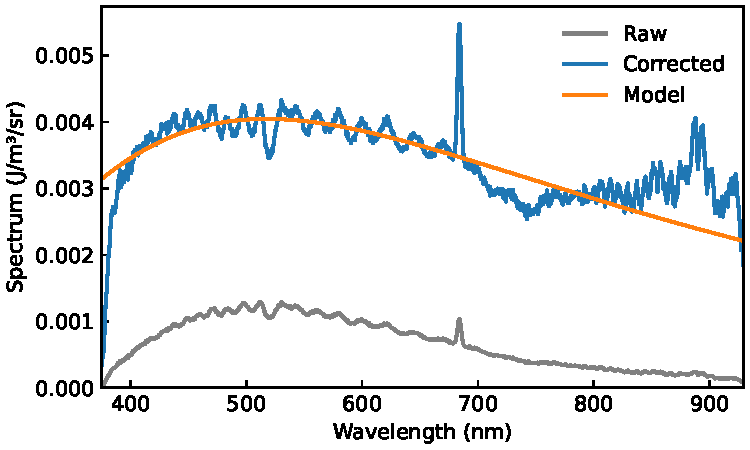
\includegraphics{../analysis/figures/combined.fit.pdf}
    \caption{Comparison of the measured spectrum and the fitted numerical model. The figure shows the raw spectrum, the spectrum corrected using the calibration curve $\eta(\lambda)$, and the resulting fitted model. The strong agreement validates the two-temperature model's applicability to the ultrafast thermal emission process.}
    \label{fig:fit}
\end{figure}

The quantitative mismatch between the model and the measurement necessitated a critical review of the fit parameters and experimental assumptions, specifically regarding two major discrepancies. First, the fitting procedure yielded a significant discrepancy in absolute magnitude, requiring a non-physical scaling factor of $0.72 \times 10^{-3}$. This indicated that the measured power was nearly three orders of magnitude lower than the absolute radiance predicted by the model. Post-measurement analysis strongly attributed this vast loss factor (in the order of $10^3$) to a severe mechanical misalignment in the detection path, specifically a blockage at the fiber coupling into the spectrometer. This suggests the scaling factor primarily reflects a systematic loss in the light collection system, rather than a fundamental deficiency in the physical model's calculated absolute emission.

Second, the inability to achieve a precise quantitative fit was compounded by spectral contamination. The corrected spectrum contained a broad, uncharacteristic light component (notably around $\SI{900}{nm}$) and a distinct peak at $\SI{688}{nm}$ (a laser harmonic). Given the absence of suitable optical filtering, this contamination was likely composed of residual laser light (fundamental and harmonic) and potentially ambient background light (e.g., neon room light). This spurious signal significantly compromised the comparison with the purely thermal model output.

Regarding the energy input, the fitted absorbed energy density, $U_{\text{abs}} = \SI{1.35}{GJ/m^3}$, is physically plausible as it is lower than the incident energy density, $U_{\text{inc}} = \SI{4.8}{GJ/m^3}$ (based on $P_{\text{avg}}=\SI{300}{mW}$, $f_{\text{rep}}=\SI{40}{kHz}$, $r_{\text{spot}}=\SI{50}{\micro m}$, and the absorption depth $d=\SI{200}{nm}$ \cite{smauszDeterminationUVVisible2017}). This difference can be attributed to surface reflections and scattering losses.


\clearpage
\section{Discussion and Conclusion}
The current work successfully applied the two-temperature model to describe the ultrafast thermal emission from hot electrons in graphite. While the qualitative agreement in the broadband spectral shape validates the general applicability of the model and its underlying physical assumptions, the analysis simultaneously revealed critical experimental and modeling limitations essential for future work.

Quantitatively, the procedure was severely hampered by the necessity of introducing a non-physical scaling factor, which indicated a systematic loss of nearly three orders of magnitude in measured power compared to the model's absolute prediction. Post-measurement analysis strongly attributes this vast discrepancy to a mechanical blockage at the spectrometer's fiber coupling, underscoring a critical systematic failure in light collection that must be fully rectified for subsequent absolute measurements.

Furthermore, the spectral fit quality was compromised by broad, uncharacteristic light components and peaks at laser harmonics. These spurious signals, likely originating from unfiltered residual laser and ambient light sources, suggest a critical deficiency in the optical filtering of the setup.

In conclusion, this study validates the two-temperature model as a robust framework in the $\SI{100}{fs}$ time regime. However, to achieve publishable results and high-precision absolute spectral power, future efforts must prioritize the rectification of the systematic collection losses and the implementation of a dedicated, traceable system calibration (e.g., using a calibration lamp).

\clearpage
\printbibliography

\end{document}